\chapter{Uso de los paquetes m\'as comunes}
\chaptertoc
\begin{objetivos}
\begin{lista}
\item Comprender el esquema básico de funcionamiento de \TeX\, y \LaTeX .
\item Conocer las diferentes salidas que produce \LaTeX.
\item Conocer las diferentes herramientas que intecactuan con \LaTeX.
\item Aprender a instalar \LaTeX\, en diferentes sistemas.
\end{lista}
\end{objetivos} 
\section{Paquetes m\'{a}s usados}
\begin{verbatim}
\usepackage[opciones]{paquete}
\end{verbatim}

\begin{description}
\item[$\square$] [spanish]\{babel\}: Espa\~{n}olizaci\'{o}n

\item[$\square$] [latin1]\{inputenc\}: Letras con acentos, e\~{n}es,

\item[$\square$] \{graphicx\}: Gr\'{a}ficos

\item[$\square$] \{amsmath\}: Macros de AMS

\item[$\square$] \{color\}: Su nombre lo indica : : :

\item[$\square$] \{hyperref\}: Hiperv\'{\i}nculos
\end{description}
\section{Fancyhdr}
\pagestyle{headings}
\subsection{Introducción}
El paquete fancyhdr se utiliza para colocar los títulos , numero páginas y cualquier otra información en la cabecera y pie de pagina de un documento.\\
Por ejemplo queremos colocar centrado en la cabecera \LaTeX , en el pie izquierdo Antalcides Olivo y en el derecho el número de la página.\\
Para logralo debemos colocar en el preámbulo
\begin{source}[Preámbulo]{c1}
\documentclass[opciones separadas por coma]{tipo de documento}
\usepackage{fancyhdr} % Cabeceras/Pies
\pagestyle{fancy} % Cabeceras/Pies
\fancyhf{} % borra todos los ajustes anteriores
\fancyhead[C]{\LaTeX}
\fancyhead[LR]{}
\fancyfoot[L]{Antalcides Olivo}
 \fancyfoot[R]{\thepage}
 \fancyfoot[C]{}
 \begin{document}
\section{Ejemplo 1}
\lipsum[1]
\end{document}
\end{source}
Obteniendo la salida \\
\begin{figure}[H]
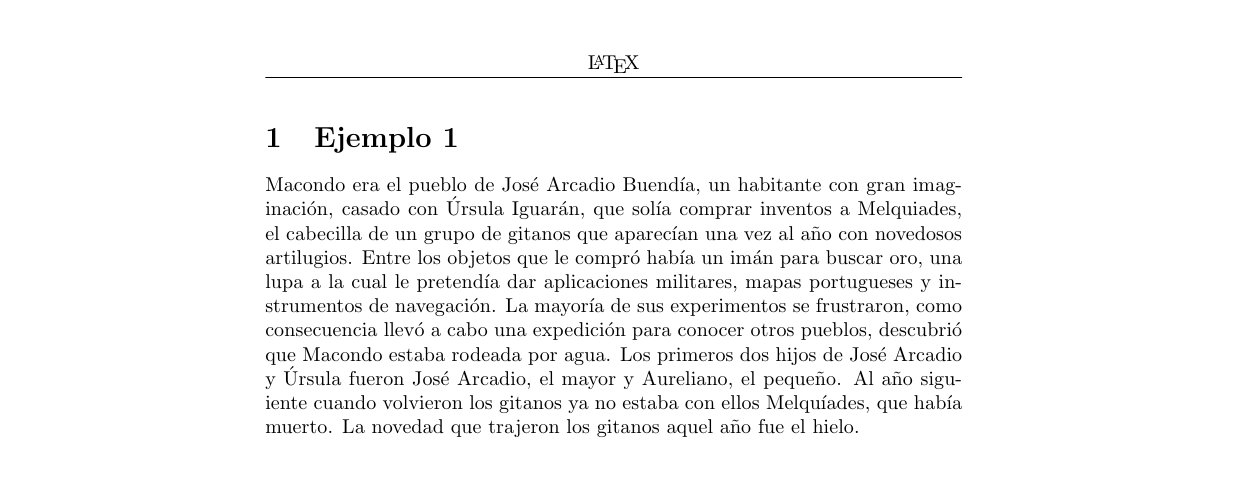
\includegraphics[scale=0.5]{salida1a.png} 
\caption{Cabecera}
\end{figure}
\begin{figure}[H]

\includegraphics[scale=0.5]{salida1b.png} 
\caption{Pie}
\end{figure}
\subsection{Uso}
\begin{lrbox}{\LstBox}
\lstinline+\documentclass[...]{...}+ y \lstinline+\begin{document}+
\end{lrbox}
Para usar el paquete \textbf{fancyhdr} tenemos que cargarlo en el preámbulo\footnote{ espacio entre \usebox{\LstBox}   } como se indica en la línea 2 del código 1.\ref{c1}, luego se empieza a personalizar el encabezado y los pie de páginas usando los comandos  \lstinline+\fancyhead[selectores]{Cabecera}+ y  \lstinline+\fancyfoot[selectores]{Pie}+ para los encabezados y pie de páginas respectivamente, con las opciones\\
\textbf{ Selectores de página}
\begin{lista}
\item E : página par
\item O: página impar
\end{lista}
\textbf{Selectores de campo}
\begin{lista}
\item L: A la izquierda
\item C: Al centro
\item R: A la derecha.
\end{lista}
Los selectores de campo y de página se pueden combinar, por ejemplo de la siguiente manera \lstinline+\fancyfoot[LE,RO]{\thepage}+ , es decir, que el pie de página aparezca a la izquierda en las pares (LE) y a la derecha en las impares (RO). Con \lstinline+\thepage+, decimos que queremos que nos aparezca el número de página. Para que se observe la diferencia entre páginas pares e impares debes colocar la opción global de la siguiente forma \lstinline+\documentclass[...,twoside]{...}+, Es posible que el texto deje de estar centrado por usar twoside, en ese caso hay que usar,\lstinline+\hoffset 0.01cm+ si queremos desplazarlo hacia la derecha un espacio de 0.01cm.\\
Para activar toda esta configuración debemos colocar en la página desde donde queramos que aparezca la configuración \lstinline+\pagestyle{fancy}+, en caso de que queramos que aparezca está configuración en todo el documento lo colocamos en el preámbulo y en la página en particular que no queremos que aparezca \lstinline+\thispagestyle{empty}+.
\subsubsection{Detalles:}
\begin{lista}
\item Si, en mitad del documento, quieres un página sin esto, usas, \lstinline+\thispagestyle{empty}+. 
\item Para limpiar los encabezados y poner otros, \lstinline+\fancyhead{}+ o \lstinline+fancyfoot{}+ o \lstinline+\fancyhf{}+.
\end{lista}
Si en alguna página específica se prefiere aplicar un estilo concreto se puede
usar \lstinline+\thispagestyle{arg}+, donde  \textbf{arg} puede ser:
\begin{lista}
\item fancy si se quiere aplicar el estilo especial
\item plain  que es el estilo por defecto es decir sin encabezado,el  pie de página contiene el número de página centrado
\item empty ninguno estilo es decir sin cabecera ni pie de página.
\item myheadings estilo sin pie de página, el encabezado contiene el número de página y la información suministrada por el usuario
\item headings sin pie de página, el encabezado contiene el nombre del capítulo y sección y / o subsección y número de página.
\end{lista}
En las cabeceras y pies de página también se puede  especificar el
número o nombre del capítulo o sección, etc. Para ello, hay que tener en cuenta que:
\begin{lista}
\item \lstinline+\leftmark+, información de nivel superior (por ejemplo, capítulo en la clase de documento book).
\item \lstinline+ \rightmark+, información de nivel inferior (p.e., sección en clase book).
\end{lista}
Estos comandos se introducen en \lstinline+\fancyhead+ o \lstinline+\fancyfoot+ sugún se requiera, por ejemplo, en un documento clase book, \lstinline+\fancyhead[LO,RE]{\leftmark}+ indica que debe aparecer el nombre del capítulo en la parte izquierda de la cabecera si es página impar, y en la derecha si es página par. Para controlar cómo se representan los capítulos, secciones, etc., en la cabecera o pie de página  del documento, se redefinen los comandos \lstinline+\chaptermark+,\lstinline+\sectionmark+,\lstinline+\subsectionmark+,etc. Antes de colocar \lstinline+\pagestyle{fancy}+ en el documento, por ejemplo:\\
El número de página es \lstinline+\thepage+. Puede aparecer en \lstinline+\fancyhead+ o \lstinline+\fancyfoot+, según se quiera; por ejemplo, \lstinline+\fancyfoot[C]{\thepage}+ indica que el número de página va aparecer centrado en el pie de todas las páginas.
\subsubsection{Lineas de adorno}
Para modificar las lineas de adorno se modifican los comandos \\
% Modifica el ancho de las líneas de cabecera y pie
\lstinline+\renewcommand{\headrulewidth}{0.4pt}+ y\lstinline+\renewcommand{\footrulewidth}{0.4pt}+ para la cabe\-cera y pie de página respectivamente.
%%%%%%%%%%%%%%%%%%%%%%%%%%%%%%%%%%%%%%%%%%%%%%%%
\subsubsection{Avanzado}
Un uso avanzado es por por ejemplo: modificando \lstinline+\chaptermark+,\lstinline+\sectionmark+,\lstinline+\subsectionmark+,etc.\\
redefiniéndolos como:\\
\lstinline+\renewcommand{\chaptermark}[1]{\markboth{\chaptername \thechapter. #1}{}}+
donde:\\
\begin{lista}
\item\lstinline+\chaptername+ = "Chapter" (por defecto) o "Capítulo"  si se ha redefinido tal como se indica en el capítulo() sección (). 
\item \lstinline+\thechapter + = número de capítulo. 
\item Observe  que \lstinline+\thechapter + va  seguido de un punto y \lstinline+#1 + este representa el argumento de \lstinline+\chaptermark+, que es el título del capítulo.
\end{lista}
Aunque el ejemplo es válido para capítulos, se hace de manera análoga para secciones \lstinline+(\sectionmark, \sectionname, \thesection), subsecciones (\subsectionmark, \subsectionname, \thesubsection},+ etc.\\
Es posible omitir alguno de los argumentos anteriores, encerrarlos entre comandos de formateo como \lstinline+\textbf{...}+ o \lstinline+\MakeUpperCase{...}+ (convertir a mayúsculas), etc dentro de los comandos \lstinline+\fancyhead{}+ o \lstinline+fancyfoot{}+.\\

NOTA: Aveces puede ser necesario ampliar el valor de altura de la cabecera \lstinline+(\headheight, por defecto, 12pt)+\lstinline+ o el pie (\footskip, por defecto 30pt)+. Esto nos lo indicará el propio \LaTeX. Para aumentar \lstinline+\headheight+ a 15pt, por ejemplo, puede usarse el comando \lstinline+\setlength{\headheight}{15pt}+ o bien \lstinline+\addtolength{\headheight}{3pt}+. También es posible aumentar o disminuir esta magnitud por un cierto factor; por ejemplo, para un incremento del 125\%: \lstinline+\setlength{\headheight}{1.25\headheight}+.
\\
También se puede cambiar el formato del número de página se establece con \lstinline+\pagenumbering{arg}+, donde arg:
\begin{lista}
\item arabic = números árabes 
\item roman = números romanos en minúscula 
\item Roman = números romanos en mayúsculas 
\item alph = letras en minúscula 
\item Alph = letras en mayúscula.
\end{lista}
Si queremos cambiar por completo las lineas de adorno las podemos redefinir como queramos, por ejemplo de la siguiente forma:
\lstinline+\renewcommand{\headrule}{\vbox to 0pt{\hbox to\headwidth{\color{gris}{\dotfill}}\vss}}+ 
Ejemplo completo\\
\begin{source}[Lineas de adorno]{c2}
\def\dayinmonth#1{%
  \ifcase#1 31\or28\or31\or30\or31\or30
            \or31\or31\or30\or31\or30\or31\fi}
\newcommand{\Today}[1][0]{%
  \advance\day by #1
  \edef\DiM{\dayinmonth{\the\month}}
  \ifnum\day>\DiM 
    \day=\numexpr \the\day-\DiM\relax 
    \advance\month\@ne
  \fi  
  \today}
\usepackage{advdate}\newcommand{\parcial}[2]{#1\, #2}
\newcommand{\porcentaje}[1]{#1\%  }
\newcommand{\materia}[1]{#1}
\newcommand{\fecha}[1]{\DayAfter[#1]}
\newcommand{\logom}[5]{\setlength{\unitlength}{1mm}
\begin{picture}(150,30)
\put(5,8){\includegraphics[width=0.2\textwidth]{/home/antalcides/.lyx/templates/LOGO1.jpg}} \put(60,15){\bf DIVISI\'ON DE
CIENCIAS B\'ASICAS} \put(60,10){\bf DEPARTAMENTO DE MATEM\'ATICAS Y
ESTAD\'ISTICA} \put(60,5){\bf \parcial{#1}{#2} \, DE \, \materia{#3\, (\porcentaje{#4})}} \put(5,0){\bf
NOMBRE:\hspace{115mm} \DayAfter[#5]}
\end{picture}}\newcommand{\logopie}{\vspace{10pt}
\begin{minipage}{0.3\textwidth}
\includegraphics[width=0.2\textwidth]{direcci\'on de la imagen}
\end{minipage}\hspace*{5mm}
\begin{minipage}{0.7\textwidth}
\bf \small Prohibido el uso de cualquier dispositivo electr\'onico con c\'amara o conexi\'on a internet y el  prest\'amo de calculadora o cualquier otro material permitido
\end{minipage}}
\fancyhf{} \clearpage
\fancyhead[C]{}
\fancyfoot{\logopie}
\end{source}
Obteniendo la salida \\
\begin{figure}[H]

\includegraphics[scale=0.5]{cabecera1.png} 
\caption{Cabecera de examen}
\end{figure}
\begin{figure}[H]
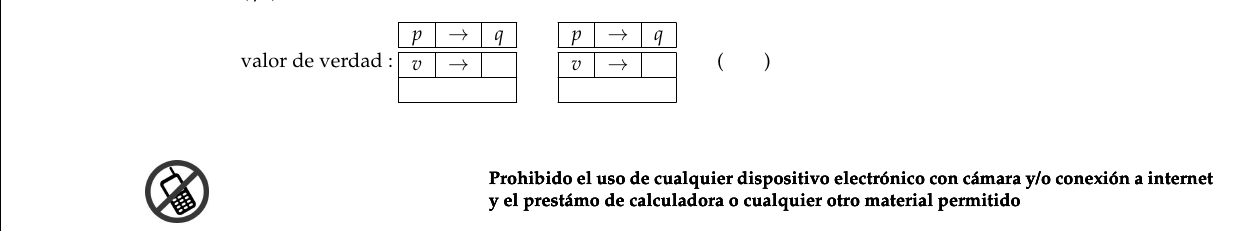
\includegraphics[scale=0.5]{pie1.png} 
\caption{Pie de examen}
\end{figure}
\begin{source}[Taller]{c4}
\renewcommand{\headrule}{
\begin{minipage}{1\textwidth}
\hrule width \hsize \kern 1mm \hrule width \hsize height 2pt 
\end{minipage}}
\renewcommand\footrule{\begin{minipage}{1\textwidth}
\hrule width \hsize height 2pt \kern 1mm \hrule width \hsize   
\end{minipage}\par}
\end{source}
\begin{figure}[H]
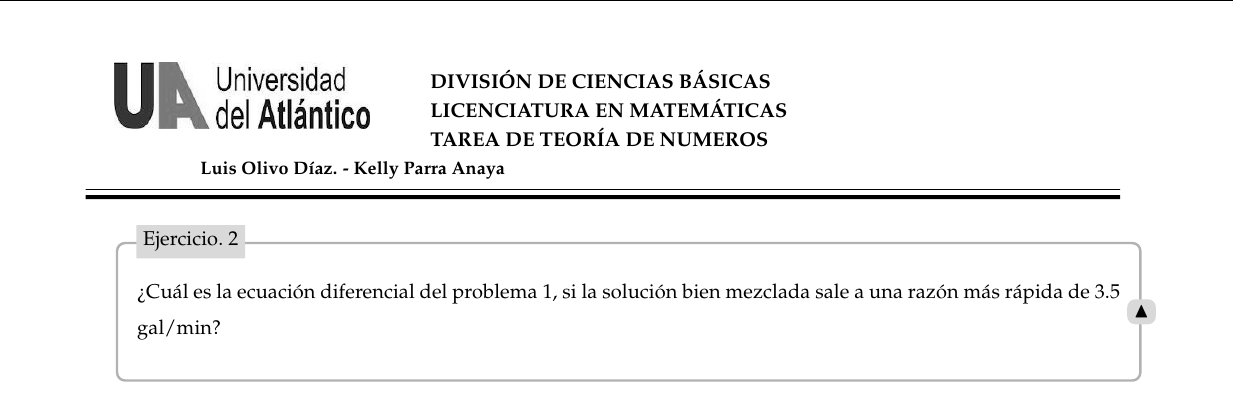
\includegraphics[scale=0.5]{cabecera2.png} 
\caption{Cabecera de tarea}
\end{figure}
%%%%%%%%%%%%%%%%%%%%%%%%%%%%%%%%%%%%%%%%%%%%
\begin{source}[Ejemplo completo]{c3}
\documentclass[...,twoside,...]{book} % Documento de clase book a dos caras
...
\usepackage{fancyhdr}
...
\pagestyle{fancy}
\fancyhf{}
\fancyhead[LO]{\leftmark} % En las p\'aginas impares, parte izquierda del encabezado, aparecer\'a el nombre de cap\'itulo
\fancyhead[RE]{\rightmark} % En las p\'aginas pares, parte derecha del encabezado, aparecer\'a el nombre de secci\'on
\fancyhead[RO,LE]{\thepage} % N\'umeros de p\'agina en las esquinas de los encabezados
\renewcommand{\chaptermark}[1]{\markboth{\textbf{\thechapter. #1}}{}} % Formato para el cap\'itulo: N. Nombre
\renewcommand{\sectionmark}[1]{\markright{\textbf{\thesection. #1}}} % Formato para la secci\'on: N.M. Nombre

\renewcommand{\headrulewidth}{0.6pt} % Ancho de la l\'inea horizontal bajo el encabezado
\renewcommand{\footrulewidth}{0.6pt} % Ancho de la l\'inea horizontal sobre el pie (que en este ejemplo est\'a vac\'io)
\setlength{\headheight}{1.5\headheight} % Aumenta la altura del encabezado en una vez y media
...
\begin{document}
... 

\end{source}